\begin{center}
  \vspace*{25pt}
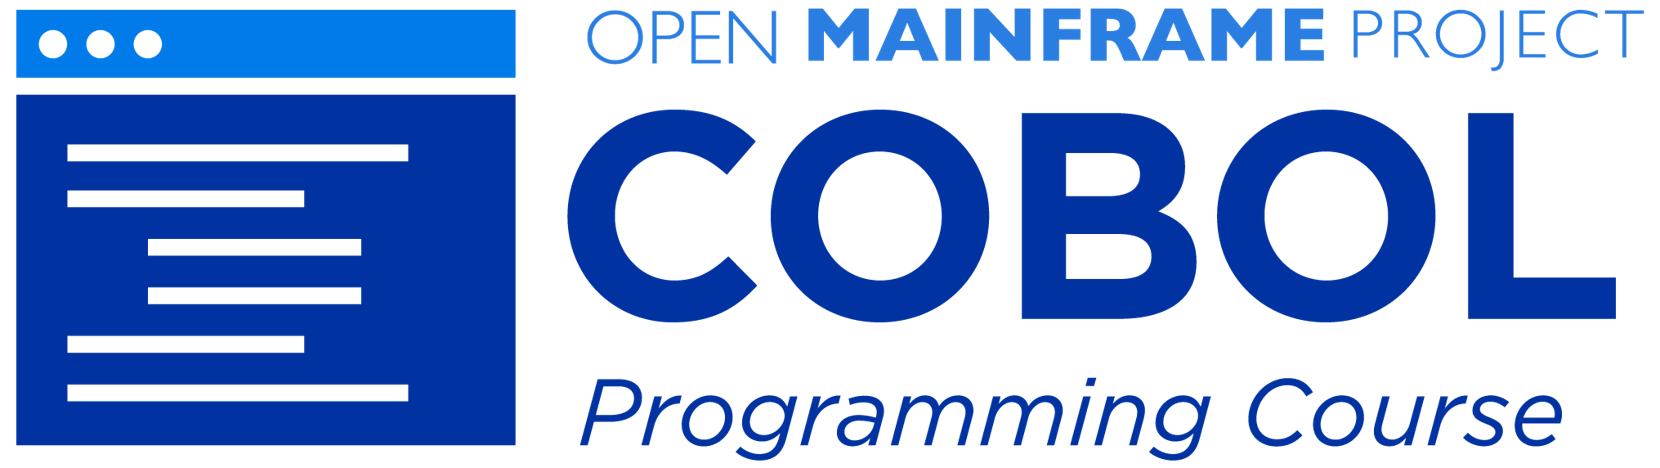
\includegraphics{Images/COBOL-Programming-Course.png}
\hypertarget{cobol-programming-course-2}{%
\section*{
  \\[35pt]
  \Huge COBOL Programming Course 2 \\[10pt]
  \Huge Learning COBOL \\[15pt]
  \Large Version 2.3.0}\label{cobol-programming-course-2}}
\end{center}

\pagebreak
\hypertarget{copyright}{%
\section*{Copyright}{
  \normalsize COBOL Programming Course is licensed under Creative Commons 
  Attribution 4.0 International. To view a copy of this license, visit 
  \href{https://creativecommons.org/licenses/by/4.0}{https://creativecommons.org/licenses/by/4.0}. \\[10pt]
  Copyright Contributors to the Open Mainframe Project's COBOL Programming Course}\label{copyright}}
\pagebreak

\hypertarget{preface}{%
\section*{Preface}\label{preface}}

\hypertarget{abstract}{%
\subsection*{Abstract}\label{abstract}}

One computer programming language was designed specifically for
business, Common Business-Oriented Language, COBOL. Today COBOL remains
as relevant as ever, handling \$3 trillion in commerce every day.

This publication is aimed at beginners looking to build a working
understanding of COBOL programming. It describes how to work with COBOL
using modern tools including Visual Studio Code with Zowe and Z Open
Editor extensions. It describes how to write, test, execute, and debug
COBOL programs.

\hypertarget{authors}{%
\subsection*{Authors}\label{authors}}

\textbf{Michael Bauer} is a development leader for the Open Mainframe
value stream at Broadcom and is a squad lead for the Zowe open source
initiative. Zowe, a popular framework of modern interfaces for z/OS,
opens the mainframe to DevOps tools and practices.  Mike leads the
Command Line Interface (CLI) squad, which created and recently spun-off
the successful Zowe Explorer extension for Visual Studio Code. A
frequent speaker and blogger, Mike runs interactive workshops around the
world for those interested in incorporating mainframe in their
enterprise DevOps initiatives.

\textbf{Ahmed Eid} is a computer engineering student from Egypt. He was 
a mentee for the Open Mainframe Project 2021 Summer Mentorship under the 
COBOL Programming Course, helping to improve the content of the course.

\textbf{Zeibura Kathau} is a technical writer for the Mainframe DevOps
value stream at Broadcom. He works on the open-source projects Che4z and 
Code4z, which are IDE extension packages for mainframe developers. He has 
8 years of experience in the Information Technology field.

\textbf{Makenzie Manna} is an IBM Redbooks Project Leader in the United
States. She has 3 years of experience in the Computer Science Software
Development field. She holds a Master's degree in Computer Science
Software Development from Marist College. Her areas of expertise include
mathematics, IBM Z and cloud computing.

\textbf{Paul Newton} is a Consulting IT Specialist in the United States.
He has 40 years of experience in the Information Technology field. He
holds a degree in Information Systems from the University of Arizona.
His areas of expertise include IBM Z, z/OS, and LinuxONE. He has written
extensively on implementation of z/OS based technology.

\textbf{Jonathan Sayles} is a technical educator at IBM, where he
conducts presentations, seminars and training courses, as well as
producing educational materials. His more than 40 years in the IT
education and computer industries encompass work within both academic
and corporate development organizations. He has also been engaged as a
software developer/designer/consultant, educator, and author, with a
focus on relational database, IDE, and object technologies. In addition
to authoring/publishing 16 books, Jon has written and published more
than 150 articles in technical journals, and served as technical editor
for several IT magazines. He is also co-author of IBM Redbook
publications Transitioning: Informix 4GL to Enterprise Generation
Language (EGL), SG24-6673 and z/OS Traditional Application Maintenance
and Support, SG24-7868.

\textbf{Hartanto Ario Widjaya} is a computer science student from 
Singapore Management University. He was a mentee for the Open Mainframe 
Project 2021 Summer Mentorship under the COBOL Programming Course, 
helping to improve the content of the course with various additions and 
assisting new learners to incorporate COBOL as a part of their tech 
toolkit.

\textbf{William Yates} is a Software engineer working for IBM UK. For
the majority of his career he has working on the CICS TS product mainly
as a software tester and now as Test Architect. He has delivered
technical content for many Redbooks, video courses and at conferences
around the world. He is also one of the leaders of the Galasa project,
building an open source integration test framework for hybrid cloud
applications available at \href{https://galasa.dev/}{https://galasa.dev}.

\hypertarget{acknowledgements}{%
\subsection*{Acknowledgements}\label{acknowledgements}}

Special thanks to the following people for participating in the
residency to shape the content in this publication.

\begin{itemize}
\item
  Dr.~Tak Auyeung, Professor, American River College
\item
  Jeffrey Bisti, Z Ecosystem Architect, IBM
\item
  Ilicena Elliott, IT Specialist II, Employment Development Department
\item
  Martin Keen, Technical Content Services, IBM
\item
  Sudharsana Srinivasan, z Influencer Ecosystem Program Coordinator, IBM
\item
  Suzy Wong, Information Technology Specialist, DMV
\item
  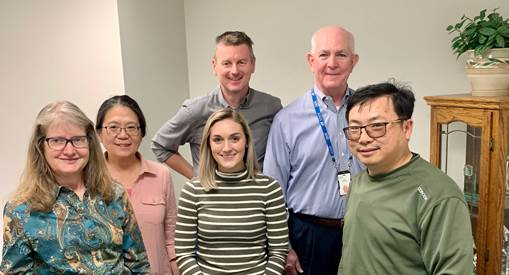
\includegraphics{Images/image004.jpg}
\end{itemize}

Left-to-right: Ilicena, Suzy, Makenzie, Martin, Paul, and Tak
\pagebreak